%!TEX root = ../thesis.tex
%*******************************************************************************
%*********************************** First Chapter *****************************
%*******************************************************************************


\chapter{Markov Processes}  %Title of the First Chapter

\ifpdf
    \graphicspath{{Chapter1/Figs/Raster/}{Chapter1/Figs/PDF/}{Chapter1/Figs/}}
\else
    \graphicspath{{Chapter1/Figs/Vector/}{Chapter1/Figs/}}
\fi

\tikzstyle{state}=[shape=circle,draw=blue!50,fill=blue!20]
\tikzstyle{observation}=[shape=rectangle,draw=orange!50,fill=orange!20]
\tikzstyle{lightedge}=[<-,dotted]
\tikzstyle{mainstate}=[state,thick]
\tikzstyle{mainedge}=[<-,thick]


%********************************** %First Section  **************************************
\section{Markov Processes} %Section - 1.1 

In order to fully understand and explore the properties and implications of Hidden Markov Models (hereinafter "HMMs") that will be used for cryptocurrency price prediction it is necessary to apriori state the underlying definition of Markov processes imminently followed by Markov Chains and finally Hidden Markov Models. 

\subsection{Definition and Properties}

Definition. Given a measurable space (S, B) called state space, where S is
a set and B is a {sigma}-algebra on S. A function P : S × B → R is called a
transition probability function if P(x, ·) is a probability measure on (S, B)
for all x  S and if for every B  B, the map s → P(s, B) is B-measurable.
Define P
1
(x, B) = P(x, B) and inductively the measures P
n+1(x, B) =
R
S
P
n(y, B)P(x, dy), where we write R








\nomenclature[z-cif]{$CIF$}{Cauchy's Integral Formula}                                % first letter Z is for Acronyms 
\nomenclature[a-F]{$F$}{complex function}                                                   % first letter A is for Roman symbols
\nomenclature[g-p]{$\pi$}{ $\simeq 3.14\ldots$}                                             % first letter G is for Greek Symbols
\nomenclature[g-i]{$\iota$}{unit imaginary number $\sqrt{-1}$}                      % first letter G is for Greek Symbols
\nomenclature[g-g]{$\gamma$}{a simply closed curve on a complex plane}  % first letter G is for Greek Symbols
\nomenclature[x-i]{$\oint_\gamma$}{integration around a curve $\gamma$} % first letter X is for Other Symbols
\nomenclature[r-j]{$j$}{superscript index}                                                       % first letter R is for superscripts
\nomenclature[s-0]{$0$}{subscript index}                                                        % first letter S is for subscripts


%********************************** %Second Section  *************************************
\section{Discrete-time Markov Chains} %Section - 1.2

Let $\Omega \neq \emptyset$ and $A \subseteq 2^{\Omega}$ be a $\sigma$-algebra on $\Omega$, and $P$ a measure on A with $P(\Omega) = 1$, i.e. $P$ is a {\it probability measure}. Then the triplet $(\Omega, A, P)$ is called a {\it probability space}. Where $\Omega$ denotes a sure event and it holds that $\forall \omega \in \Omega$ is called an elementary event. Furthermore, $\forall A \in A$ is a random event  so that $P(A)$ is a probability of such a random event. 

Let $I$ be a countable set and $\Theta$ a $\sigma$-algebra on $I$. Each $i \in I$ is called a {\it state} and $(I,\Theta)$ a {\it state-space}. We say that $\lambda = (\lambda_i : i \in I) $ is a measure on I if $0 \leq \lambda_i \leq \infty$. If in addition the {\it total mass} $\sum_{i \in I} \lambda_i = 1$ then $\lambda$ is a {\it distribution} (or probability measure). 

Suppose now that we have two measurable spaces $(\Omega,A)$ and $(I,\Theta)$ and a random variable $X: \Omega \rightarrow I$ assuming that X is measurable. Thus we call $(I,\Theta)$ a state space and $(\Omega, A)$ an underlying space. Therefore we may set:

\begin{equation}
\lambda_X(i) = P(X=i)=P(\{\omega: X(\omega)=i\})
\end{equation}

Since we are allowing only for the discrete realisations of the random variable X, given previous assumptions, $\lambda_X(i)$ is a {\it probability mass function}.

Then measure $\lambda$ defines a distribution of $X$. Given such a setting random variable $X$ is assumed to denote random state $i$ with probability $\lambda_i$. 

To simply illustrate the idea behind discrete Markov Chains let us assume a situation where the future market movements transition between a countable number of states $I =$ \{upward movement, no movement, downward movement\} and there is a transition matrix (also called {\it stochastic matrix}) $P = (p_{i,j} : i,j \in I)$ defined as:
\begin{equation*}
P =
\begin{pmatrix}
0.1 & 0.4 & 0.5 \\
0.25 & 0.3 & 0.45 \\
0.33 & 0.33 & 0.33 
\end{pmatrix}
\end{equation*}
Each row represents full set of transition probabilities between each state which is visible from $\sum_{j \in I} ^{}p_{i,j} = 1 $, i.e. each row of matrix $P$ represents a full distribution of transitions over $I$. Such a relationship can be represented as a diagram indexing each state by A, B and C respectively as follows:

\begin{center}
\begin{tikzpicture}[->, >=stealth', auto, semithick, node distance=3cm]
\tikzstyle{every state}=[fill=white,draw=black,thick,text=black,scale=1]
\node[state]    (A)                     {$A$};
\node[state]    (B)[right of=A]   {$B$};
\node[state]    (C)[right of=B]   {$C$};

\path
(A) edge[loop left]     node{$0.1$}         (A)
    edge[bend left,below]     node{$0.4$}     (B)
    edge[bend right,below]      node{$0.5$}      (C)
(B) edge[bend left,below]     node{$0.45$}           (C)
    edge[loop below]     node{$0.3$}           (B)
    edge[bend left, above]     node{$0.25$}           (A)
(C) edge[bend right,above] node{$0.33$}           (A)
    edge[loop right]     node{$0.33$}         (C)
    edge[bend left, above]      node{$0.33$}         (B);
\end{tikzpicture}
\end{center}
 
This may be easily interpreted for each given state. For example if we assume that the market moved upwards on the last trading day there is a 0.1 chance that the market will move in positive direction today, in other words the conditional probability of observing the state A today given the state A yesterday is 0.1. On the hand if we suppose that today the market actually transitioned to the state B  with probability 0.4 there is now a probability of 0.45 to transition to state C since the future transition is only conditioned by its previous state. 

Till now we have assumed random variable X that modelled the probability of observing a state $i \in I$ given the initial distribution $\lambda$. We ought to consider  thus we have to allow for a system of discrete random variables that are also identically distributed for each time step $\{X_{t},t \in T \}$, for $\{t_0,t_1,...,t_n\} \subset T$ where $n \in \mathbb{N}_0$.

Suppose now that we have observed a given sequence of states for the last week as $\{A,B,C,C,A\}$ and we would like to know its probability of observing given the transition matrix P and distribution $\lambda$. Then $P(X_{t_0},...,X_{t_n}|P,\lambda)$ can be calculated as:

\begin{align*}
P(X_{t_0},...,X_{t_n}|P,\lambda) &= P(A,B,C,C,A|P,\lambda) \\
&= P(A) * P(B|A) * P(C|B) * P(C|C) * P(A|C) \\
&= \lambda * p_{1,2} * p_{2,3} * p_{3,3} * p_{3,1} \\
&= \lambda * 0.4 * 0.45 * 0.33 * 0.33
\end{align*}

maybe bych tam dal product of Xs

Where the probability of observing state A is determined by our distribution $\lambda$ evaluated at respective state A since we have no prior knowledge about what exactly happened before $t_0$. 

On the other hand, we might consider a situation in which we have observed such a sequence of events and we need to determine the next state given the sequence. As in the last example, we have our transition matrix P, distribution $\lambda$ and a sequence of events observed until now $\{A,B,C,C,A\}$ for $t_{k-4},...,t_{k}$. Let us also assume that $t_{k+1}$ is a time of next event for which we are trying to determine its probability.

\begin{align}
P(X_{t_{k+1}}|X_{t_{k}},...,X_{t_{k-4}}) &= P(X_{t_{k+1}}|X_{t_{k}})
\end{align}

We know that last observed state was A which directs us straight to the first row of our transition matrix P since from the properties of Markov Processes (the process is memoryless) we know that the next state will depend solely on the present state so we can abstract from the given sequence of past states and focus only on $X_{t_{k}}$. Finally we may conclude that the most likely future state is C with probability of 0.5. 

Obviously, the probabilities in previous transition matrix P were imaginary and served only as a mere example of the main properties of Discrete-time Markov Chains. From now on we consider a dataset of BTC-USD daily close prices calculated my CoinMarketCap website from 5th March 2017 to 5th March 2022. FIrst of all we ought to make several assumptions about the data in order to apply the logic and properties of Markov Chains. 

Assumption 1: The close daily prices of BTC-USD trading pair are discrete, meaning that we only record prices at exactly 0:00 of each day since there are no closing hours of the major cryptocurrency exchanges. This assumption will be elevated in the next section with Continous-time Markov Chains.

Assumption 2: We will assume that future prices of Bitcoin depend only on their pre





Theorems:





%********************************** % Third Section  *************************************
\section{Continous-time Markov Chains}  %Section - 1.3 
\label{section1.3}

















Viterbi algorithm should, in its most general form, provide a solution to the maximum a posteriori probability (MAP) estimation of the state sequence of a finite-state discrete-time Markov process introduced in the last chapter. 


\section{Hidden Markov Model}

Up until now we have considered visible states in a sense that the sequence of states was known, we refer to these models as $visible$ $Markov$ $Models$. In this section we will consider a situation in which we do not observe the states directly but only as a guess given other visible observations that are available to us. These "visible" observations are considered as an emissions from the hidden state sequence. Thus, the observations are assumed to be generated by the hidden states. We may interpret this relation by the following diagram where we have a hidden state sequence $Z = \{z_1, z_2,...z_T\}$:

\begin{figure}[htbp]
\begin{center}
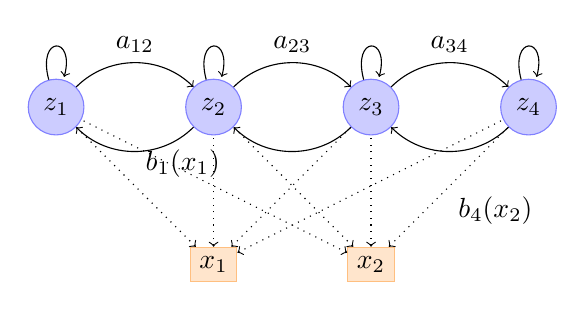
\begin{tikzpicture}[]
% states
\node[state] (s1) at (0,2) {$z_1$}
    edge [loop above]  ();
\node[state] (s2) at (2,2) {$z_2$}
    edge [<-,bend right=45] node[auto,swap] {$a_{12}$} (s1)
    edge [->,bend left=45] (s1)
    edge [loop above] ();
\node[state] (s3) at (4,2) {$z_3$}
    edge [<-,bend right=45] node[auto,swap] {$a_{23}$} (s2)
    edge [->,bend left=45] (s2)
    edge [loop above] ();
\node[state] (s4) at (6,2) {$z_4$}
    edge [<-,bend right=45] node[auto,swap] {$a_{34}$}  (s3)
    edge [->,bend left=45] (s3)
    edge [loop above] ();
% observations
\node[observation] (y1) at (2,0) {$x_1$}
    edge [lightedge] node[auto,swap] {$b_1(x_1)$} (s1)
    edge [lightedge] (s2)
    edge [lightedge] (s3)
    edge [lightedge] (s4);
\node[observation] (y2) at (4,0) {$x_2$}
    edge [lightedge] (s1)
    edge [lightedge] (s2)
    edge [lightedge] (s3)
    edge [lightedge] node[auto,swap] {$b_4(x_2)$} (s4);
\end{tikzpicture}
\end{center}
\caption{An HMM with 4 hidden states which emits 2 discrete observable states denoted by $x_1$ or $x_2$.
$a_{ij}$ is the probability to transition from state $z_i$ to state $z_j$.
$b_j(x_k)$ is the probability to emit symbol $x_k$ in state $z_j$.}
\end{figure}

There are 3 main assumptions of Hidden Markov Models as a consequence of the properties of Markov processes. For $Z = \{z_t\}_{t=0}^T$ being the hidden state sequence:

\begin{itemize}
\item[1)] The Markov assumption - this assumption states that the next hidden state $z_{t+1}$ depends only on the current state $z_t$, so that the transition probabilities are defined as:

\begin{equation}
P(z_{t+1} = j| z_{t} = i,z_{t-1} = l,...,z_{0} = n) = P(z_{t+1} = j| z_{t} = i) = p_{ij}
\end{equation}

It it also possible to assume that the states in HMM are dependant beyond the current state therefore giving rise to k-order HMMs as opposed to classical first-order HMM, moreover, such variations are uneasy to analyse.

\item[2)] The stationarity assumption - The transition matrix is invariant of the time, thus for any arbitrarily set time $t_1$ and $t_2$:

\begin{equation}
P(z_{t_1+1} = j| z_{t_1}) = P(z_{t_2+1} = j| z_{t_2} = i) = p_{ij}
\end{equation}

\item[3)] The observation independence assumption - The current observation or output is statistically independent of the previous observations. So if we have a observation sequence $X = \{x_1,x_2,...,x_T\}$ then:

\begin{equation}
P(X|z_1,z_2,...,z_T, \lambda) = \prod_{t=1}^T P(x_t|z_t,\lambda)
\end{equation}

\end{itemize}

Given these assumptions we define the joint probability of the hidden states and the observations $P(X,Z)$ as follows:

\begin{equation}
P(X, Z) = \prod_{t=1}^T P(z_t|z_{t-1}) P(x_t|z_t)
\end{equation}



There are mainly 3 fundamental problems in HMM that need to be resolved as in (Oliver C. Ibe):

\begin{itemize}
\item[1.] Evaluation problem - Given a model denoted as $\lambda = (P,\theta,\pi)$ and an observation sequence $X = x_1, x_2,...,x_T$, how to efficiently compute the probability that the model generated the observation sequence, in other words, what is $P(X|\lambda)$? 
\item[2.] Decoding problem - Given a model $\lambda = (P,\theta,\pi)$, what is the most likely sequence of hidden states that could have generated a given observation sequence? Thus we would like to find $Z = \underset{Z}{\arg\max} P(Z,X|\lambda)$, where $Z$ is the hidden state sequence. 
\item[3.] The learning problem - Given a set of observation sequences find the HMM that best explains the observation sequence. Thus, find the values of $\lambda$ that maximise $P(X|\lambda)$ or in order to estimate the most likely parameters of HMM for a given observation sequence. 
\end{itemize}

The most traditional approaches in solving these 3 fundamental problems differ and one may not suffice in solving all three. The evaluation problem is usually by forward-backward algorithm, the decoding problem by well-known Viterbi algorithm and the last learning problem by Baum-Welsch algorithm which is a special case of Expectation-maximization (EM) algorithm. 

\subsection{Forward and Backward algorithm}

While given a sequence of observations, in our case observable states, denoted by $X = x_1,x_2,...,x_T$ and a model $\lambda = (P,\theta,\pi)$ we wold like to compute the conditional probability of observing the sequence $X$ under the model constraints. Thus:

 \begin{equation}
P(X| \lambda) = \sum_Z P(X|Z,\lambda)*P(Z|\lambda)
\end{equation}

where $Z = z_1,z_2,...,z_T$ is a fixed sequence of hidden states. Our goal may be divided into two parts while the first part $P(X|Z,\lambda)$ computes the conditional probability of the observation sequence X given the sequence Z and model $\lambda$ and the second part $P(Z|\lambda)$ accounts only for the transition probabilities among the hidden states. To summarise:

\begin{align}
P(X| Z, \lambda) &= \prod_{t=1}^T  P(x_t|z_t,\lambda) = \theta_{z_1}(x_1) \prod_{t=2}^T \theta_{z_t}(x_t) \\ \nonumber
P(Z|\lambda)&= \pi_{z_1} * \prod_{t=2}^{T} p_{z_t z_{t+1}}
\end{align}

where $\theta_{z_t}(x_t)$ is the emission probability from observation $x_t$ into $z_t$ in our model and $p_{z_t z_{t+1}}$ are the transition probabilities for the given sequence Z. After substitution of terms from Eq. 1.8 into Eq 1.7 we obtain:

\begin{align}
P(X| \lambda) &= \sum_Z P(X|Z,\lambda)*P(Z|\lambda) \\ \nonumber
&= \sum_{z_1,...,z_T}\theta_{z_1}(x_1) \pi_{z_1} \prod_{t=2}^{T} p_{z_t z_{t+1}} \theta_{z_t}(x_t)
\end{align}

The summation above refers to all possible permutations of the sequence of hidden states Z which implies that we would have $N^T$ possible sequences if we assume that $N$ indicates all possible hidden states at each step. Furthermore, in order to calculate $P(X|\lambda)$ we have $2TN^T$ calculations which is exponential in T and not feasible for real application. As opposed to brute-force procedure as described above we take use of a forward and backward algorithm. 

\subsubsection{Forward algorithm}

Previous introduction required huge amounts of calculations that were essentially unnecessary, redundant. Each sequence can be decomposed into multiple subsequences which are shared among different sequences and do not need to be recomputed again. These subsequences can be represented by a trellis as shown in Fig 1.2. With a help of such diagram we may imagine recording the probability of each distinct subsequence at each time step. In other words, we wish to compute the joint probability $P(z_t,x_1,x_2,...,x_t)$ while taking advantage of the conditional independence of $x_t$ which only depends on $z_t$, moreover, due to Markov assumption, $z_t$ depends only on $z_{t-1}$. Let us now define the forward probability variable $\alpha_t(i)$ as follows:

 \begin{equation}
\alpha_t(i) = P(x_1,x_2,...,x_{t-1},x_t,z_t=i |\lambda)
\end{equation}

Which we may also define as the probability of being in state i at time t after having observed the sequence ${x_1,x_2,...,x_t}$. The calculation therefore results in summing the incoming arcs at trellis node which is derived from:

\begin{align}
\alpha_t(i) &= P(x_1,x_2,...,x_{t-1},x_t,z_t=i |\lambda) \\ \nonumber
&= P(x_t|z_t=I, \lambda) P(x_1,x_2,...,x_{t-1},z_t=i |\lambda)  \\ \nonumber
&= P(x_t|z_t=i, \lambda) \sum_{j \in I} P(z_t = I| z_{t-1}=j,\lambda) P(x_1,x_2,...,x_{t-1},z_{t-1}=j |\lambda) \\ \nonumber
&= \theta_i(x_t) \sum_{j=1}^N p_{ji} \alpha_{t-1}(j)
\end{align}

Where $I$ is a set of all possible hidden states, $i,j$ denote elements of $I$ and $N$ the size of set $|I|$. We would repeat the iterative procedure until the termination at time T where $P(X|\lambda) = \sum_{i=1}^N  \alpha_T(i) = \sum_{i=1}^N P(X,z_T=I|\lambda)$. Moreover, we initialise the trellis with $\alpha_1(i)=\pi_i \theta_i(x_1)$. Resulting algorithm requires time complexity of $O(TN^2)$ which is a significant improvement from the brute force approach with complexity of $O(2TN^T)$.
  
\begin{figure}[htbp]
\begin{center}
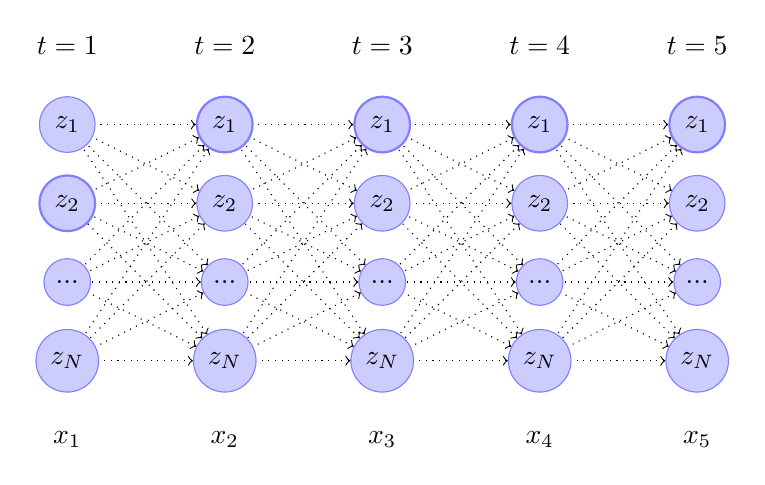
\begin{tikzpicture}[]
% 1st column
\node               at (0,6) {$t=1$};
\node[state] (s1_1) at (0,5) {$z_1$};
\node[mainstate] (s2_1) at (0,4) {$z_2$};
\node[state] (s3_1) at (0,3) {$...$};
\node[state] (s4_1) at (0,2) {$z_N$};
\node at (0,1) {$x_1$};
% 2nd column
\node               at (2,6) {$t=2$};
\node[mainstate] (s1_2) at (2,5) {$z_1$}
    edge[lightedge] (s1_1)
    edge[lightedge] (s2_1)
    edge[lightedge] (s3_1)
    edge[lightedge] (s4_1);
\node[state] (s2_2) at (2,4) {$z_2$}
    edge[lightedge] (s1_1)
    edge[lightedge] (s2_1)
    edge[lightedge] (s3_1)
    edge[lightedge] (s4_1);
\node[state] (s3_2) at (2,3) {$...$}
    edge[lightedge] (s1_1)
    edge[lightedge] (s2_1)
    edge[lightedge] (s3_1)
    edge[lightedge] (s4_1);
\node[state] (s4_2) at (2,2) {$z_N$}
    edge[lightedge] (s1_1)
    edge[lightedge] (s2_1)
    edge[lightedge] (s3_1)
    edge[lightedge] (s4_1);
\node at (2,1) {$x_2$};
% 3rd column
\node               at (4,6) {$t=3$};
\node[mainstate] (s1_3) at (4,5) {$z_1$}
    edge[lightedge]  (s1_2)
    edge[lightedge] (s2_2)
    edge[lightedge] (s3_2)
    edge[lightedge] (s4_2);
\node[state] (s2_3) at (4,4) {$z_2$}
    edge[lightedge] (s1_2)
    edge[lightedge] (s2_2)
    edge[lightedge] (s3_2)
    edge[lightedge] (s4_2);
\node[state] (s3_3) at (4,3) {$...$}
    edge[lightedge] (s1_2)
    edge[lightedge] (s2_2)
    edge[lightedge] (s3_2)
    edge[lightedge] (s4_2);
\node[state] (s4_3) at (4,2) {$z_N$}
    edge[lightedge] (s1_2)
    edge[lightedge] (s2_2)
    edge[lightedge] (s3_2)
    edge[lightedge] (s4_2);
\node at (4,1) {$x_3$};
% 4th column
\node               at (6,6) {$t=4$};
\node[mainstate] (s1_4) at (6,5) {$z_1$}
    edge[lightedge]  (s1_3)
    edge[lightedge] (s2_3)
    edge[lightedge] (s3_3)
    edge[lightedge] (s4_3);
\node[state] (s2_4) at (6,4) {$z_2$}
    edge[lightedge] (s1_3)
    edge[lightedge] (s2_3)
    edge[lightedge] (s3_3)
    edge[lightedge] (s4_3);
\node[state] (s3_4) at (6,3) {$...$}
    edge[lightedge] (s1_3)
    edge[lightedge] (s2_3)
    edge[lightedge] (s3_3)
    edge[lightedge] (s4_3);
\node[state] (s4_4) at (6,2) {$z_N$}
    edge[lightedge] (s1_3)
    edge[lightedge] (s2_3)
    edge[lightedge] (s3_3)
    edge[lightedge] (s4_3);
\node at (6,1) {$x_4$};
% 5th column
\node               at (8,6) {$t=5$};
\node[mainstate] (s1_5) at (8,5) {$z_1$}
    edge[lightedge]  (s1_4)
    edge[lightedge] (s2_4)
    edge[lightedge] (s3_4)
    edge[lightedge] (s4_4);
\node[state] (s2_5) at (8,4) {$z_2$}
    edge[lightedge] (s1_4)
    edge[lightedge] (s2_4)
    edge[lightedge] (s3_4)
    edge[lightedge] (s4_4);
\node[state] (s3_5) at (8,3) {$...$}
    edge[lightedge] (s1_4)
    edge[lightedge] (s2_4)
    edge[lightedge] (s3_4)
    edge[lightedge] (s4_4);
\node[state] (s4_5) at (8,2) {$z_N$}
    edge[lightedge] (s1_4)
    edge[lightedge] (s2_4)
    edge[lightedge] (s3_4)
    edge[lightedge] (s4_4);
\node at (8,1) {$x_5$};
\end{tikzpicture}
\end{center}
\caption{Trellis of the observation sequence $x_1$,...,$x_5$ for the above HMM. As an example, the transition between state $z_1$ at time t=2 and state $z_4$ at time t=3 has probability $\alpha_2(z_1)p_{14}\theta_{z_4}(x_3)$, where $\alpha_t(i)$ is the probability to be instate $i$ at time t.}
\end{figure}

\pagebreak

\subsubsection{Backward algorithm}

While computing the backward probability variable denoted as $\beta_t(i)$ we assume the reversed iterative procedure. Let us define the backward probability variable as:

\begin{align}
\beta_t(i) &= P(x_{t+1},x_{t+2},...,x_{t-1},x_t|z_t=i ,\lambda) \\ \nonumber
&= \sum_{i,j \in I} P(x_{t+1},x_{t+2},...,x_{t-1},x_t,z_{t+1}=j|z_t=i ,\lambda)   \\ \nonumber
&= \sum_{i,j \in I} P(x_{t+1}|z_{t+1}=j) P(x_{t+2},...,x_{t-1},x_t|z_{t+1}=j) P(z_{t+1}=j|z_{t}=i,\lambda) \\ \nonumber
&= \sum_{j=1}^N \theta_j(x_{t+1})p_{ij} \beta_{t+1}(j)
\end{align}

As we could have in forward algorithm we define effectively 3 steps:

\begin{itemize}
\item[1.] Initialization step: with default value of $\beta_T(i) = 1$ for $i \in {1,2,...,N}$. 
\item[2.] Induction step: 

\begin{equation}
\beta_t(i) = \theta_j(x_{t+1})p_{ij} \beta_{t+1}(j)
\end{equation}

Afterwards, we update the time t = t-1 and check whether expression above holds which is as long as t $>$ 0.
\item[3.] Termination step: once the iterative procedure is exhausted, i.e. when t=0 we have the estimate of $P(X|\lambda)$ as:

\begin{equation}
P(X|\lambda) = \sum_{j=1}^N \theta_j(x_{1})\pi_{i} \beta_{1}(i) = \sum_{j=1}^N \alpha_1(i)  \beta_{1}(i)
\end{equation}

\end{itemize}

Getting everything together we may prove that the forward and backward algorithms coincide in solving the posterior joint and marginal distributions of all hidden states. Consider the case of posterior joint distribution:

\begin{align}
P(X|\lambda) &= \sum_{i=1}^N P(X,z_t=i|\lambda) \\ \nonumber
&= \sum_{i=1}^N P(x_1,x_2,...,x_{t},x_{t+1},...,x_{T}|z_t=i,\lambda) P(z_t = i|\lambda) \\ \nonumber
&= \sum_{i=1}^N P(x_1,x_2,...,x_{t}|z_t=i,\lambda) P(x_{t+1},...,x_{T}|z_t=i,\lambda) P(z_t = i|\lambda) \\ \nonumber
&= \sum_{i=1}^N P(x_1,x_2,...,x_{t},z_t=i|\lambda) P(x_{t+1},...,x_{T}|z_t=i,\lambda) \\ \nonumber
&= \sum_{i=1}^N \alpha_{t}(i) \beta_t(i) 
\end{align}

See that above we take a use of conditional independence of observations given the hidden state and therefore we may transform the problem using already known variables for forward and backward passes over the hidden states. Thus, the posterior marginal distribution is:

\begin{equation}
P(X, z_t=i|\lambda) = \alpha_t(i) \beta_t(i)
\end{equation}

\subsection{Viterbi algorithm}

Once we solve the evaluation problem, thus finding the optimal procedure in computing the posterior marginal distributions of all hidden states and $P(X|\lambda)$, we may visualise the result in a trellis as shown in Figure 1.2. The second problem, decoding problem, aims to find the sequence of hidden states $Z^*$ that most likely produced observation sequence $X$. Finding the most likely sequence $Z^*$ maximazes $P(Z|X,\lambda)$. As in the encoding problem, the complexity of the optimisation problem explodes if we decide to compute all possible sequences of hidden states to $N^T$ calculations. The solution as in the forward and backward algorithm simplifies when we calculate the hidden state with highest probability individually rather than entire sequence up to time $t$. The idea is that once we find the most likely hidden state given observation and the model at each time step we may discard the rest of the possible hidden states since they obviously could not have most likely produced the observation. The complexity of the optimal sequence of hidden states decreases significantly to $NT$ thus transforming the exponential complexity into linear. As in forward and backward algorithm we define variable $\gamma_t(i)$ as:

\begin{equation}
\gamma_t(i) = P(z_t=i|X,\lambda) = \frac{P(X,z_t=i|\lambda)}{P(X|\lambda)} =\frac{\alpha_t(i) \beta_t(i)}{\sum_{i=1}^N \alpha_t(i) \beta_t(i)} \propto \alpha_t(i) \beta_t(i)
\end{equation}

Where the expressions in the third equality are obtained as a solution to a before mentioned equations. Also, the $P(X|\lambda)$ serves only as a normalising constant and is irrelevant for the optimisation given the respective time step. Moreover, the conditional probability $\gamma_t(i)$ forms a conditional probability mass function since it is non-negative for all possible values of hidden states and observations and the sum over all possible hidden states at each time step is:

\begin{equation}
\sum_{i=1}^N  \gamma_t(i) = 1
\end{equation}

This would be one of the possible ways to estimate the most likely hidden states individually and then combine them sequentially to obtain the whole sequence of hidden states as:

\begin{equation}
z_t^* = \underset{i \in I}{\arg\max} \{\gamma_t(i)\}
\end{equation}

Method as described by the Eq 1.17 and 1.19 is also called maximum a posteriori probability estimate (hereinafter "MAP estimate") which equals to the mode of the posterior distribution. If the posterior distribution is discrete, the mode is simply the value of a random variable with the highest probability. For continuous distributions the mode is a value of a random variable for which the likelihood/log-likelihood function attains its local maximum/maxima. Assuming now $Z$ denotes the continuous random variable of hidden states and observation sequence $X$ up to time t is present, the MAP estimate of the hidden state $\hat{Z}_{MAP}$ at a given point in time is:

\begin{align}
\hat{z}_{t,MAP} &= \underset{z_t}{\arg\max} \: f(Z_t|X) \\ \nonumber
&= \underset{z_t}{\arg\max} \: \frac{f(X|Z_t)g(Z_t)}{\int_{I} f(X|Z_t)g(Z_t) \,dZ} \\ \nonumber
&= \underset{z_t}{\arg\max} \: f(X|Z_t)g(Z_t)\\ \nonumber
\end{align}

Where $g$ indicates probability density function of $Z_t$, so called prior distribution, and $I$ is its domain. The second equality follows from the Bayes' Theorem. The result clearly holds for the discrete case:

\begin{align}
\hat{z}_{t,MAP} &= \underset{z_t}{\arg\max} \: P(Z_t=i|X) \\ \nonumber
&= \underset{z_t}{\arg\max} \: \frac{P(X|Z_t=i)P(Z_t=i)}{\sum_{i=1}^N P(X|Z_t=i)P(Z_t=i)} \\ \nonumber
&= \underset{z_t}{\arg\max} \:P(X|Z_t=i)P(Z_t=i)\\ \nonumber
&= z_t^*\\ \nonumber
\end{align}

However, the solution as such might not produce the most likely sequence of states given the sequence of observations. This is due to the fact that the individual estimates do not incorporate the transition probability between most likely states at time t-1 and t. Hence, it might be possible that some states are highly unlikely to transition into other that were evaluated as most likely. Fortunately, the mentioned shortcomings of such approach are easily solved by Viterbi algorithm.

In order to find the most likely sequence of hidden states $Z^*={z_1^*,z_2^*,...,z_T^*}$ given the observation sequence $X={x_1,x_2,...,x_T}$ it is necessary to maximise with respect to the whole sequence rather than individually to avoid less likely transitions as introduced. The algorithm therefore defines a variable as follows:

\begin{equation}
\delta_t(i) = \underset{Z_{t-1}}{\max}\:P(z_1,z_2,...,z_t=i,x_1,x_2,...,x_{t-1},x_{t}|\lambda)
\end{equation}

That is the most likely state sequence given the observation sequence up to time $t$. Moreover, for the purpose of the algorithm we also define variable $\psi_t(i)$ that stores the node of the incoming arc that leads to the most probable state path.

\begin{equation}
\psi_t(j) = \underset{i \in I}{\arg\max} \: \delta_{t-1}(i)p_{ij}
\end{equation}

\vspace{0.3cm}

\noindent
Then we can easily provide the steps to obtain the most likely state sequence:

\begin{itemize}
\item[1.] Initialize the algorithm given the initial distribution of hidden states $\pi$:

\begin{align}
\delta_1(i) &= \pi_i b_i(o_1)  \\
\psi_1(i)& = 0
\end{align}

where we compute the initial values of above variables for each hidden state $i \in I$.

\item[2.] Recursive step:

\begin{align}
\delta_1(i) &= \underset{i \in I}{\arg\max} \: \delta_{t-1}(i)p_{ij} b_j(o_t)  \\
\psi_t(j)& = \underset{i \in I}{\arg\max} \: \delta_{t-1}(i)p_{ij}
\end{align}

At each iterative step we update the time so that $t=t+1$. The second step continues as long as the $t<T$ if that does not hold the third step terminates the algorithm and we backtrack the most likely state sequence. Although, recursive step is very similar to the induction step in the forward algorithm there exist a main difference between the two that lies in the fact that Viterbi algorithm uses maximization instead of summation over previous states. 

\item[3.] Termination step for the last observation 

\begin{align}
P^* &= \underset{i \in I}{\max} \: \delta_{T}(i) \\
q_T^* & = \underset{i \in I}{\arg\max} \: \delta_{T}(i)
\end{align}

\item[4.] Backtrack the optimal state sequence:

\begin{equation}
z_t^* = \psi_{t+1}(z_{t+1}^*)
\end{equation}

For $t = T-1,T-2,...,1$.

\end{itemize}

The resulting most likely state path can be visually viewed as in the form of a path within the trellis introduced in Fig. 1.2:

\begin{figure}[htbp]
\begin{center}
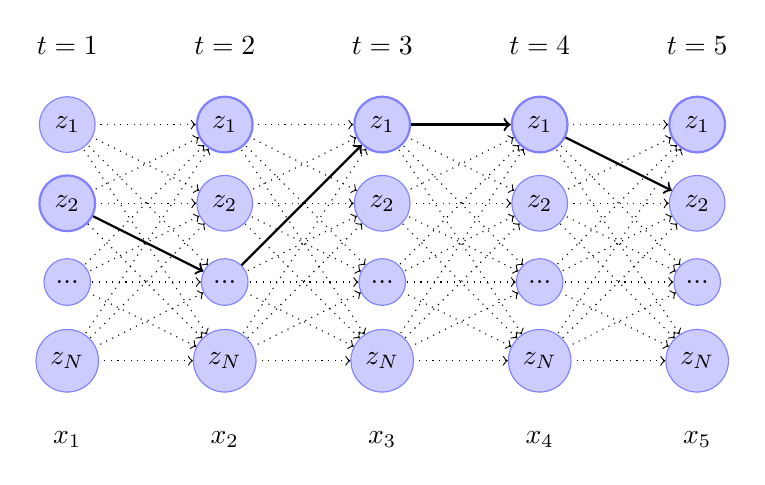
\begin{tikzpicture}[]
% 1st column
\node               at (0,6) {$t=1$};
\node[state] (s1_1) at (0,5) {$z_1$};
\node[mainstate] (s2_1) at (0,4) {$z_2$};
\node[state] (s3_1) at (0,3) {$...$};
\node[state] (s4_1) at (0,2) {$z_N$};
\node at (0,1) {$x_1$};
% 2nd column
\node               at (2,6) {$t=2$};
\node[mainstate] (s1_2) at (2,5) {$z_1$}
    edge[lightedge] (s1_1)
    edge[lightedge] (s2_1)
    edge[lightedge] (s3_1)
    edge[lightedge] (s4_1);
\node[state] (s2_2) at (2,4) {$z_2$}
    edge[lightedge] (s1_1)
    edge[lightedge] (s2_1)
    edge[lightedge] (s3_1)
    edge[lightedge] (s4_1);
\node[state] (s3_2) at (2,3) {$...$}
    edge[lightedge] (s1_1)
    edge[mainedge] (s2_1)
    edge[lightedge] (s3_1)
    edge[lightedge] (s4_1);
\node[state] (s4_2) at (2,2) {$z_N$}
    edge[lightedge] (s1_1)
    edge[lightedge] (s2_1)
    edge[lightedge] (s3_1)
    edge[lightedge] (s4_1);
\node at (2,1) {$x_2$};
% 3rd column
\node               at (4,6) {$t=3$};
\node[mainstate] (s1_3) at (4,5) {$z_1$}
    edge[lightedge]  (s1_2)
    edge[lightedge] (s2_2)
    edge[mainedge] (s3_2)
    edge[lightedge] (s4_2);
\node[state] (s2_3) at (4,4) {$z_2$}
    edge[lightedge] (s1_2)
    edge[lightedge] (s2_2)
    edge[lightedge] (s3_2)
    edge[lightedge] (s4_2);
\node[state] (s3_3) at (4,3) {$...$}
    edge[lightedge] (s1_2)
    edge[lightedge] (s2_2)
    edge[lightedge] (s3_2)
    edge[lightedge] (s4_2);
\node[state] (s4_3) at (4,2) {$z_N$}
    edge[lightedge] (s1_2)
    edge[lightedge] (s2_2)
    edge[lightedge] (s3_2)
    edge[lightedge] (s4_2);
\node at (4,1) {$x_3$};
% 4th column
\node               at (6,6) {$t=4$};
\node[mainstate] (s1_4) at (6,5) {$z_1$}
    edge[mainedge]  (s1_3)
    edge[lightedge] (s2_3)
    edge[lightedge] (s3_3)
    edge[lightedge] (s4_3);
\node[state] (s2_4) at (6,4) {$z_2$}
    edge[lightedge] (s1_3)
    edge[lightedge] (s2_3)
    edge[lightedge] (s3_3)
    edge[lightedge] (s4_3);
\node[state] (s3_4) at (6,3) {$...$}
    edge[lightedge] (s1_3)
    edge[lightedge] (s2_3)
    edge[lightedge] (s3_3)
    edge[lightedge] (s4_3);
\node[state] (s4_4) at (6,2) {$z_N$}
    edge[lightedge] (s1_3)
    edge[lightedge] (s2_3)
    edge[lightedge] (s3_3)
    edge[lightedge] (s4_3);
\node at (6,1) {$x_4$};
% 5th column
\node               at (8,6) {$t=5$};
\node[mainstate] (s1_5) at (8,5) {$z_1$}
    edge[lightedge]  (s1_4)
    edge[lightedge] (s2_4)
    edge[lightedge] (s3_4)
    edge[lightedge] (s4_4);
\node[state] (s2_5) at (8,4) {$z_2$}
    edge[mainedge] (s1_4)
    edge[lightedge] (s2_4)
    edge[lightedge] (s3_4)
    edge[lightedge] (s4_4);
\node[state] (s3_5) at (8,3) {$...$}
    edge[lightedge] (s1_4)
    edge[lightedge] (s2_4)
    edge[lightedge] (s3_4)
    edge[lightedge] (s4_4);
\node[state] (s4_5) at (8,2) {$z_N$}
    edge[lightedge] (s1_4)
    edge[lightedge] (s2_4)
    edge[lightedge] (s3_4)
    edge[lightedge] (s4_4);
\node at (8,1) {$x_5$};
\end{tikzpicture}
\end{center}
\caption{Trellis of the observation sequence $x_1$,...,$x_5$ for the HMM. Bold lines illustrate the most likely sequence found by the Viterbi algorithm.}
\end{figure}


\newpage


\section{Kalman Filters}




\nomenclature[z-DEM]{DEM}{Discrete Element Method}
\nomenclature[z-FEM]{FEM}{Finite Element Method}
\nomenclature[z-PFEM]{PFEM}{Particle Finite Element Method}
\nomenclature[z-FVM]{FVM}{Finite Volume Method}
\nomenclature[z-BEM]{BEM}{Boundary Element Method}
\nomenclature[z-MPM]{MPM}{Material Point Method}
\nomenclature[z-LBM]{LBM}{Lattice Boltzmann Method}
\nomenclature[z-MRT]{MRT}{Multi-Relaxation Time}
\nomenclature[z-RVE]{RVE}{Representative Elemental Volume}
\nomenclature[z-GPU]{GPU}{Graphics Processing Unit}
\nomenclature[z-SH]{SH}{Savage Hutter}
\nomenclature[z-CFD]{CFD}{Computational Fluid Dynamics}
\nomenclature[z-LES]{LES}{Large Eddy Simulation}
\nomenclature[z-FLOP]{FLOP}{Floating Point Operations}
\nomenclature[z-ALU]{ALU}{Arithmetic Logic Unit}
\nomenclature[z-FPU]{FPU}{Floating Point Unit}
\nomenclature[z-SM]{SM}{Streaming Multiprocessors}
\nomenclature[z-PCI]{PCI}{Peripheral Component Interconnect}
\nomenclature[z-CK]{CK}{Carman - Kozeny}
\nomenclature[z-CD]{CD}{Contact Dynamics}
\nomenclature[z-DNS]{DNS}{Direct Numerical Simulation}
\nomenclature[z-EFG]{EFG}{Element-Free Galerkin}
\nomenclature[z-PIC]{PIC}{Particle-in-cell}
\nomenclature[z-USF]{USF}{Update Stress First}
\nomenclature[z-USL]{USL}{Update Stress Last}
\nomenclature[s-crit]{crit}{Critical state}
\nomenclature[z-DKT]{DKT}{Draft Kiss Tumble}
\nomenclature[z-PPC]{PPC}{Particles per cell}